\documentclass[reqno,11pt]{amsart}
\usepackage{math327-lecture}
\usepackage{needspace}
\usepackage{tikz}
\lectureinfo{20}{Oct. 26, 2026}{Quotient Groups and the First Isomorphism Theorem}
\artinsections{2.12}

% Typeset from handwritten Lecture 14, Oct. 3, 2025, pp. 1--14.
\begin{document}
\makelecturetitle

\section{The quotient group}

Let $N\trianglelefteq G$. The elements of $G/N$ are the left cosets
$gN$. In general such a space of cosets is just a set, but under the normal condition we can say more.

We define their product by
\[
  (g_1N)(g_2N)=(g_1g_2)N.
\]

The first point is to note that this product does not depend on the
representatives of the cosets.

\begin{proposition}\label{prop:well-defined}
The multiplication above is well defined on $G/N$.
\end{proposition}
\begin{proof}
Suppose $g_1N=\widetilde g_1N$ and
$g_2N=\widetilde g_2N$. Then
\[
  \widetilde g_1^{-1}g_1\in N,
  \qquad \widetilde g_2^{-1}g_2\in N.
\]
We need to show that $g_1g_2N=\widetilde g_1\widetilde g_2N$.
Indeed,
\[
  (\widetilde g_1\widetilde g_2)^{-1}g_1g_2
  =\widetilde g_2^{-1}(\widetilde g_1^{-1}g_1)g_2
  =\underbrace{\widetilde g_2^{-1}(\widetilde g_1^{-1}g_1)
       \widetilde g_2}_{\in N}
    \underbrace{\widetilde g_2^{-1}g_2}_{\in N}
  \in N.
\]
The first factor belongs to $N$ by normality, so the resulting
cosets are equal.
\end{proof}

The operation is associative because multiplication in $G$ is
associative. Its identity is $N=1N$, and the inverse of $gN$ is
$g^{-1}N$:
\[
  (gN)(1N)=(1N)(gN)=gN,
  \qquad (gN)(g^{-1}N)=N.
\]

\begin{theorem}[Quotient group and quotient map]\label{thm:quotient-group}\label{thm:quotient-map}
Let $N\trianglelefteq G$. Then:
\begin{enumerate}[label=\textup{(\alph*)}]
\item The coset multiplication
$(g_1N)(g_2N)=(g_1g_2)N$ makes $G/N$ a group.
\item The map
\[
  \pi:G\longrightarrow G/N,\qquad g\longmapsto gN,
\]
is a surjective homomorphism with $\ker\pi=N$.
\end{enumerate}
\end{theorem}
\begin{proof}
The group axioms in part~(a) were checked above. For part~(b), by the
definition of coset multiplication,
\[
  \pi(g_1g_2)=(g_1g_2)N=(g_1N)(g_2N)
  =\pi(g_1)\pi(g_2).
\]
Also, $gN=N$ exactly when $g\in N$, so $\ker\pi=N$.
Every coset is $\pi(g)$ for some $g\in G$; hence
$\im\pi=G/N$.
\end{proof}

How can one identify the quotient group? Often if you think you know the answer, you can use the following result.


\begin{theorem}[First isomorphism theorem]\label{thm:first-iso}
Let $\varphi:G\to G'$ be a homomorphism and put $N=\ker\varphi$.
Then
\[
  G/N\cong\im\varphi.
\]
More precisely, the isomorphism is
\[
  \overline\varphi:G/N\longrightarrow\im\varphi,
  \qquad gN\longmapsto\varphi(g),
\]
and $\varphi=\overline\varphi\circ\pi$.
\end{theorem}
\begin{proof}
The kernel $N$ is normal in $G$, so $G/N$ is a group.
To check that $\overline\varphi$ is well defined, observe that
\begin{align*}
  gN=\widetilde gN
  &\iff \widetilde g^{-1}g\in N=\ker\varphi\\
  &\iff \varphi(\widetilde g^{-1}g)=1\\
  &\iff \varphi(g)=\varphi(\widetilde g).
\end{align*}
It is a homomorphism, since
\[
  \overline\varphi((g_1N)(g_2N))
  =\varphi(g_1g_2)
  =\varphi(g_1)\varphi(g_2)
  =\overline\varphi(g_1N)\overline\varphi(g_2N).
\]
It is surjective onto $\im\varphi$ by definition of the image.
If $\overline\varphi(gN)=1$, then $g\in\ker\varphi=N$, so
$gN=N$. Hence it is injective. Finally,
$\overline\varphi(\pi(g))=\varphi(g)$ for every $g\in G$.
\end{proof}

For a surjective homomorphism $\varphi:G\to G'$, this reads
$G/\ker\varphi\cong G'$. The theorem also applies when $\varphi$
is not surjective, provided that the target of the induced
isomorphism is $\im\varphi$.



The quotient group makes every element of $N$ equal to the identity.
For example, if $a_1,\ldots,a_r\in G$ and
$a_1\cdots a_r\in N$, then in $G/N$ we have
\[
(a_1N)\cdots(a_rN)=(a_1\cdots a_r)N=N=1_{G/N}.
\]
Thus a product of elements of $G$ that lies in $N$ becomes the
identity in the quotient. The universal property describes exactly
which homomorphisms from $G$ descend to $G/N$.


\begin{theorem}[Universal property]\label{thm:universal-quotient}
Let $N\trianglelefteq G$, let $\pi:G\to G/N$ be the quotient map,
and let $f:G\to H$ be a homomorphism. There is a homomorphism
$\overline f:G/N\to H$ such that $f=\overline f\circ\pi$ if and
only if $N\subseteq\ker f$. When it exists, $\overline f$ is unique
and is given by
\[
  \overline f(gN)=f(g).
\]
Thus the following diagram commutes:
\[
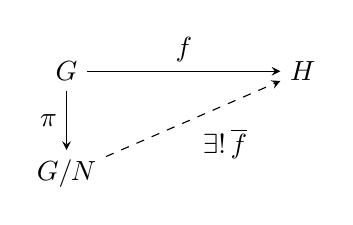
\begin{tikzpicture}[baseline=(current bounding box.center),>=stealth]
  \node (G) at (0,1.3) {$G$};
  \node (Q) at (0,0) {$G/N$};
  \node (H) at (3,1.3) {$H$};
  \draw[->] (G)--node[above] {$f$} (H);
  \draw[->] (G)--node[left] {$\pi$} (Q);
  \draw[->,dashed] (Q)--node[below right] {$\exists!\,\overline f$} (H);
\end{tikzpicture}
\]
\end{theorem}
\Needspace{7\baselineskip}
\begin{proof}
If $f=\overline f\circ\pi$ and $n\in N$, then
$f(n)=\overline f(N)=1_H$, so $N\subseteq\ker f$.

Conversely, suppose $N\subseteq\ker f$. If $gN=g'N$, then
$(g')^{-1}g\in N$, hence $f(g')^{-1}f(g)=1_H$.
Thus $f(g)=f(g')$, so the formula
$\overline f(gN)=f(g)$ is well defined. Moreover,
\[
  \overline f\bigl((gN)(hN)\bigr)
  =f(gh)=f(g)f(h)=\overline f(gN)\overline f(hN),
\]
so $\overline f$ is a homomorphism, and
$\overline f(\pi(g))=f(g)$ for every $g\in G$.
Finally, any map satisfying $f=\overline f\circ\pi$ must send
$gN=\pi(g)$ to $f(g)$. Since $\pi$ is surjective, this determines
$\overline f$ uniquely.
\end{proof}

The inclusion $N\subseteq\ker f$ allows a map out of $G/N$
to send additional cosets to the identity. If $N=\ker f$, the
induced map is injective and gives
the first isomorphism theorem after restricting its codomain
to $\im f$.

\section{Examples}

\begin{example}[Integers modulo $n$]\label{ex:integers-mod-n}
Let $n\geq1$. Since $(\Z,+)$ is abelian, $n\Z\trianglelefteq\Z$.
The quotient group is
\[
  \Z/n\Z=\{\overline0,\overline1,\ldots,\overline{n-1}\},
  \qquad \overline a=a+n\Z,
\]
with addition
\[
  \overline a+\overline b=\overline{a+b}.
\]
Two integers give the same coset exactly when their difference
is divisible by $n$. The identity is $\overline0$, the inverse
of $\overline a$ is $\overline{-a}$, and $\overline1$ generates
the group, so $\Z/n\Z$ is cyclic of order $n$.
For example, in $\Z/5\Z$,
$\overline3+\overline4=\overline7=\overline2$.

The quotient map is $\pi:\Z\to\Z/n\Z$, $a\mapsto\overline a$,
with kernel $n\Z$. To illustrate the universal property, choose
$h\in H$ and define $f:\Z\to H$ by $f(a)=h^a$.
Then $f$ factors through $\Z/n\Z$ exactly when $h^n=1_H$.
In that case the unique induced homomorphism is
\[
  \overline f:\Z/n\Z\longrightarrow H,
  \qquad \overline a\longmapsto h^a.
\]
\end{example}

\begin{example}[The determinant]
The determinant is a surjective homomorphism
\[
  \det:\GL_n(\R)\longrightarrow\R^\times,
  \qquad A\longmapsto\det A,
\]
where $\R^\times=\R\setminus\{0\}$ under multiplication.
It is surjective because
$\det(\operatorname{diag}(r,1,\ldots,1))=r$ for every
$r\in\R^\times$. Its kernel is
$\SL_n(\R)=\{A\in\GL_n(\R):\det A=1\}$. Therefore
\[
  \GL_n(\R)/\SL_n(\R)\cong\R^\times.
\]
\end{example}

\begin{example}
Every normal subgroup is a kernel: if $N\trianglelefteq G$, then
$N=\ker\pi$ for the quotient map $\pi:G\to G/N$.
For example, the sign homomorphism
$\sgn:S_n\to\{\pm1\}$ has kernel $A_n$. For $n\geq2$ it is
surjective, so
\[
  S_n/A_n\cong\{\pm1\}.
\]
The identity $G/\ker\varphi\cong\im\varphi$ applies even when
$\varphi$ is not surjective onto its stated codomain.
\end{example}

\Needspace{18\baselineskip}
\begin{example}[A quotient of $S_4$]
Let
\[
  V=\{1,(12)(34),(13)(24),(14)(23)\}.
\]
Recall the action of $S_4$ on the three partitions of
$\{1,2,3,4\}$ into two unordered pairs:
\[
  P_1=\{12\mid34\},\qquad
  P_2=\{13\mid24\},\qquad
  P_3=\{14\mid23\}.
\]
This action gives a homomorphism $\varphi:S_4\to S_3$, where
$S_3$ permutes the labels $1,2,3$ of the partitions. For example,
\[
  \varphi((12))=(23),\qquad \varphi((123))=(132).
\]
A transposition and a $3$-cycle generate $S_3$, so $\varphi$ is
surjective. Each element of $V$ fixes all three partitions, so
$V\subseteq\ker\varphi$. The counting formula gives
$|\ker\varphi|=24/6=4$, hence $\ker\varphi=V$.
Thus $V\trianglelefteq S_4$, and the first isomorphism theorem gives
\[
  S_4/V\cong S_3,\qquad \sigma V\longmapsto\varphi(\sigma).
\]
In particular, this quotient has six elements, each a coset of size four.
\end{example}

\Needspace{18\baselineskip}
\begin{example}[An upper triangular matrix group]
Let
\[
  H=\left\{
   \begin{pmatrix}1&a&b\\0&1&c\\0&0&1\end{pmatrix}
   :a,b,c\in\R\right\},\qquad
  K=\left\{
   \begin{pmatrix}1&0&x\\0&1&0\\0&0&1\end{pmatrix}
   :x\in\R\right\}.
\]
Write $M(a,b,c)$ for the displayed matrix in $H$.
Matrix multiplication gives
\[
  M(a,b,c)M(a',b',c')
  =M(a+a',\,b+b'+ac',\,c+c'),
\]
Also,
\[
  M(a,b,c)^{-1}=M(-a,ac-b,-c).
\]
Thus $H$ is a subgroup of $\GL_3(\R)$. it is easy to see that $K$ is a subgroup of $H$, and in fact it is normal in $H$: indeed,
$M(a,b,c)M(0,x,0)=M(a,b+x,c)=M(0,x,0)M(a,b,c)$,
so $K$ is central in $H$, i.e. $K$ commutes with everything in $H$. 

Naively, we would expect $H/K$ to be two dimensional, and expressed in terms ot the two coordinates $a$ and $c$. How to make this precise ? Use the first isomorphism theorem and define
\[
  \varphi:H\longrightarrow (\R,+)\times(\R,+),
  \qquad M(a,b,c)\longmapsto(a,c).
\]
The multiplication formula shows that $\varphi$ is a homomorphism.
It is surjective, and its kernel is precisely $K$. Hence
\[
  H/K\cong(\R,+)\times(\R,+).
\]
\end{example}

\end{document}
